\chapter{Scraper Design and Implementation - IHPScrape}\label{C:us}

In this section the design and implementation of the web scraping components of the project are discussed. Important decisions made during the course of the project are highlighted, as well as steps taken to implement the system based upon the requirements detailed in Chapter 4.

% I highlight important decisions made during the course of the project, as well as steps taken to implement the system based on requirements detailed in chapter four.

%\section{A Prototyping Approach}

%Talk about how the design was constructed.

%My approach to prototyping and the problems this revealed.

%The overall design of my scrapers was largely developed through a prototyping approach early in the project. I performed research and web-scraping frameworks and technologies to decide which would best suit the requirements defined in chapter 4. The prototyping strategy also allowed me to investigate the feasibility of scraping from different sites.

%By developing prototypes for Facebook and Twitter early in the project I was better able to 

\section{Architecture}

Two potential architectures were considered when designing the web-scraper components.

\begin{itemize}
 \item A database storage approach
 \item A text/XML storage approach
\end{itemize}



%The database approach was ultimately rejected, and the more straightforward text/XML design used. The database design added unnecessary complexity and time-investment to develop the framework. The performance cost of saving to a database rather than a file also 

%The reason for this rejection was due to a database design adding unnecessary complexity to the application, as well as time required to develop the framework. The performance cost of saving to a database was also unnecessary, so this over-engineered solution was rejected. 

%Having received feedback on the database approach, the more straightforward and suitable text/XML design was ultimately used.

\subsection{Database Storage Architecture}

\begin{figure}[h!]
\begin{center} 
 \centering
  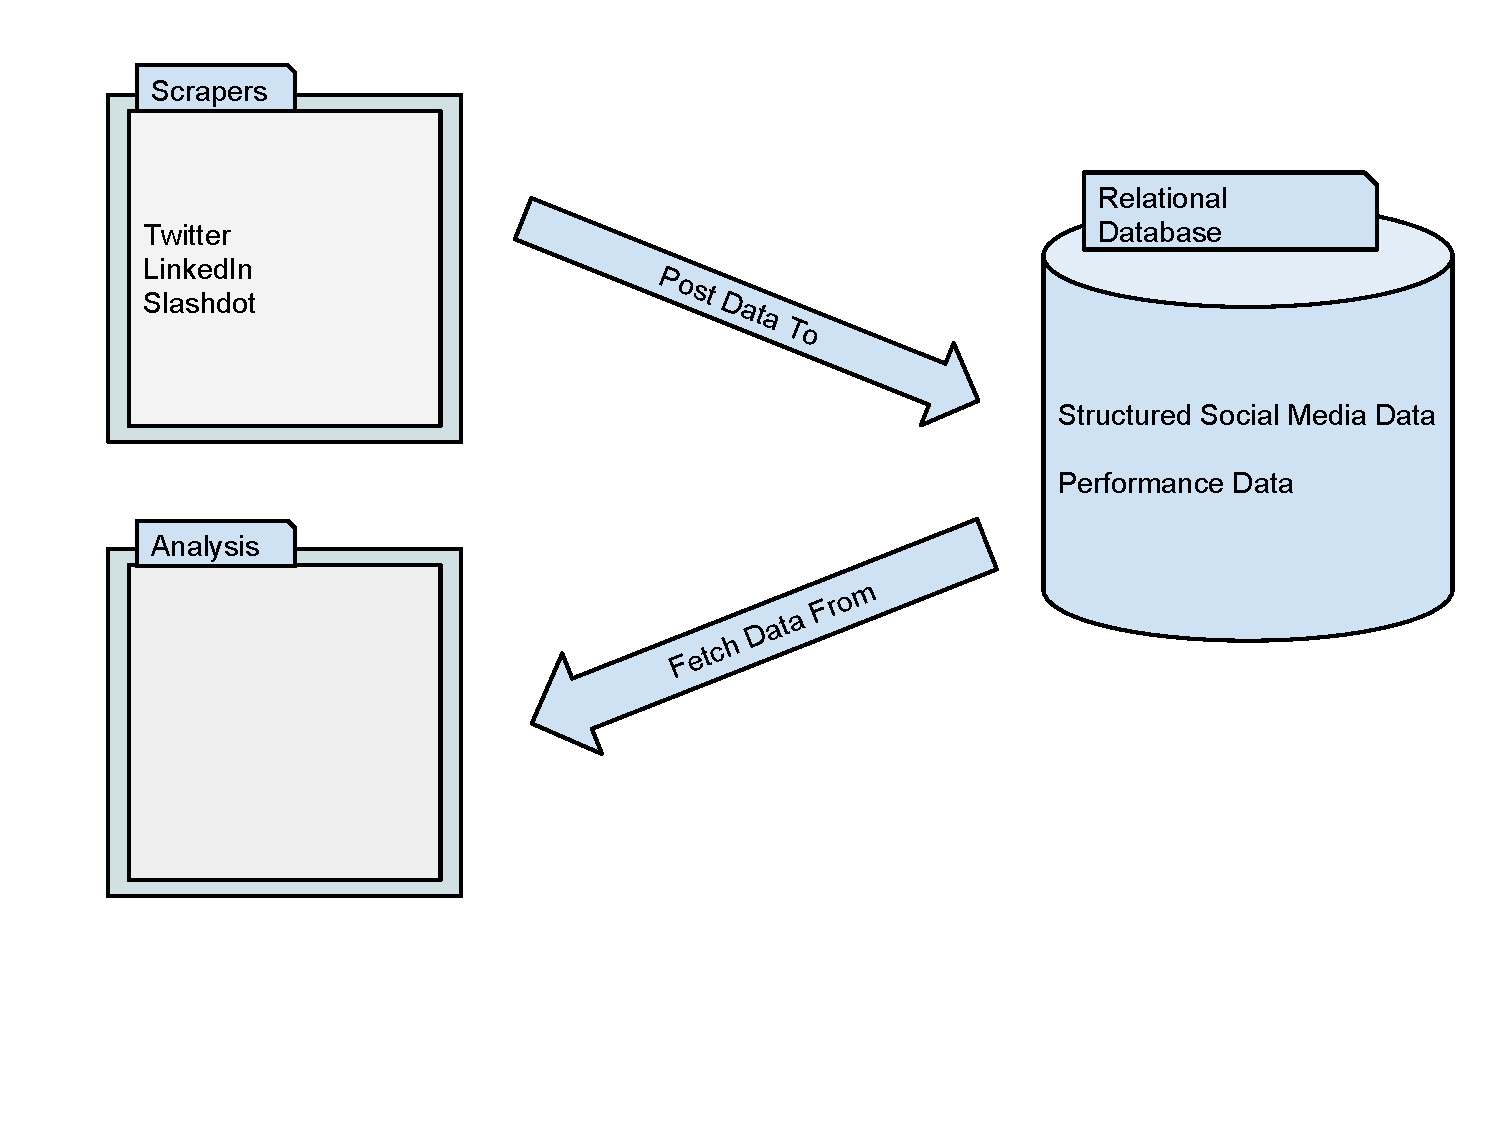
\includegraphics[width=0.9\textwidth]{Images/Database_Architecture.pdf}
 \caption{Proposed Architecture for Database Storage Solution}
 \label{fig:database_storage}
\end{center}
 \end{figure}

A possible approach to meeting the requirements of the project was to store fetched data in a relational database. As shown in Figure \ref{fig:database_storage}, the scrapers would gather data over an extended period of time, writing retrieved information into a database. Analysis components would then fetch data from the database as necessary, saving results in separate tables within the same schema.

This approach provides long-term extensibility benefits, as per requirement F3. All of the advantages that come with database storage would have been present in this solution -
specifically selection of individual profile elements and updates to these elements would have been more straightforward. However this design was deemed to be over-engineered for the purposes of the project. Given that data retrieved is in HTML, JSON or XML format there is a large impedance mismatch between retrieved data and relational database tuple format. This is compounded when retrieving data from the store for analysis - many third party analysis tools require input data in a variety of text forms.  The analysis components were also largely contingent on the fetching of a whole profile, rather than specific elements, lessening the need for querying against specific elements in my data storage structure. 

\subsection{XML Storage Architecture}

An alternative architecture involves the scraper and analysis components interacting with a shared XML storage system. As shown in Figure \ref{fig:xml_storage}, scrapers run over time whilst saving data to a common XML-based file system. Analysis components could then annotate and enrich the original dataset. Note that analysis components in this architecture essentially act as source nodes for the GRAft system, through generating some reputation metrics associated with a profile. 

\begin{figure}[h!]
\begin{center}
\centering
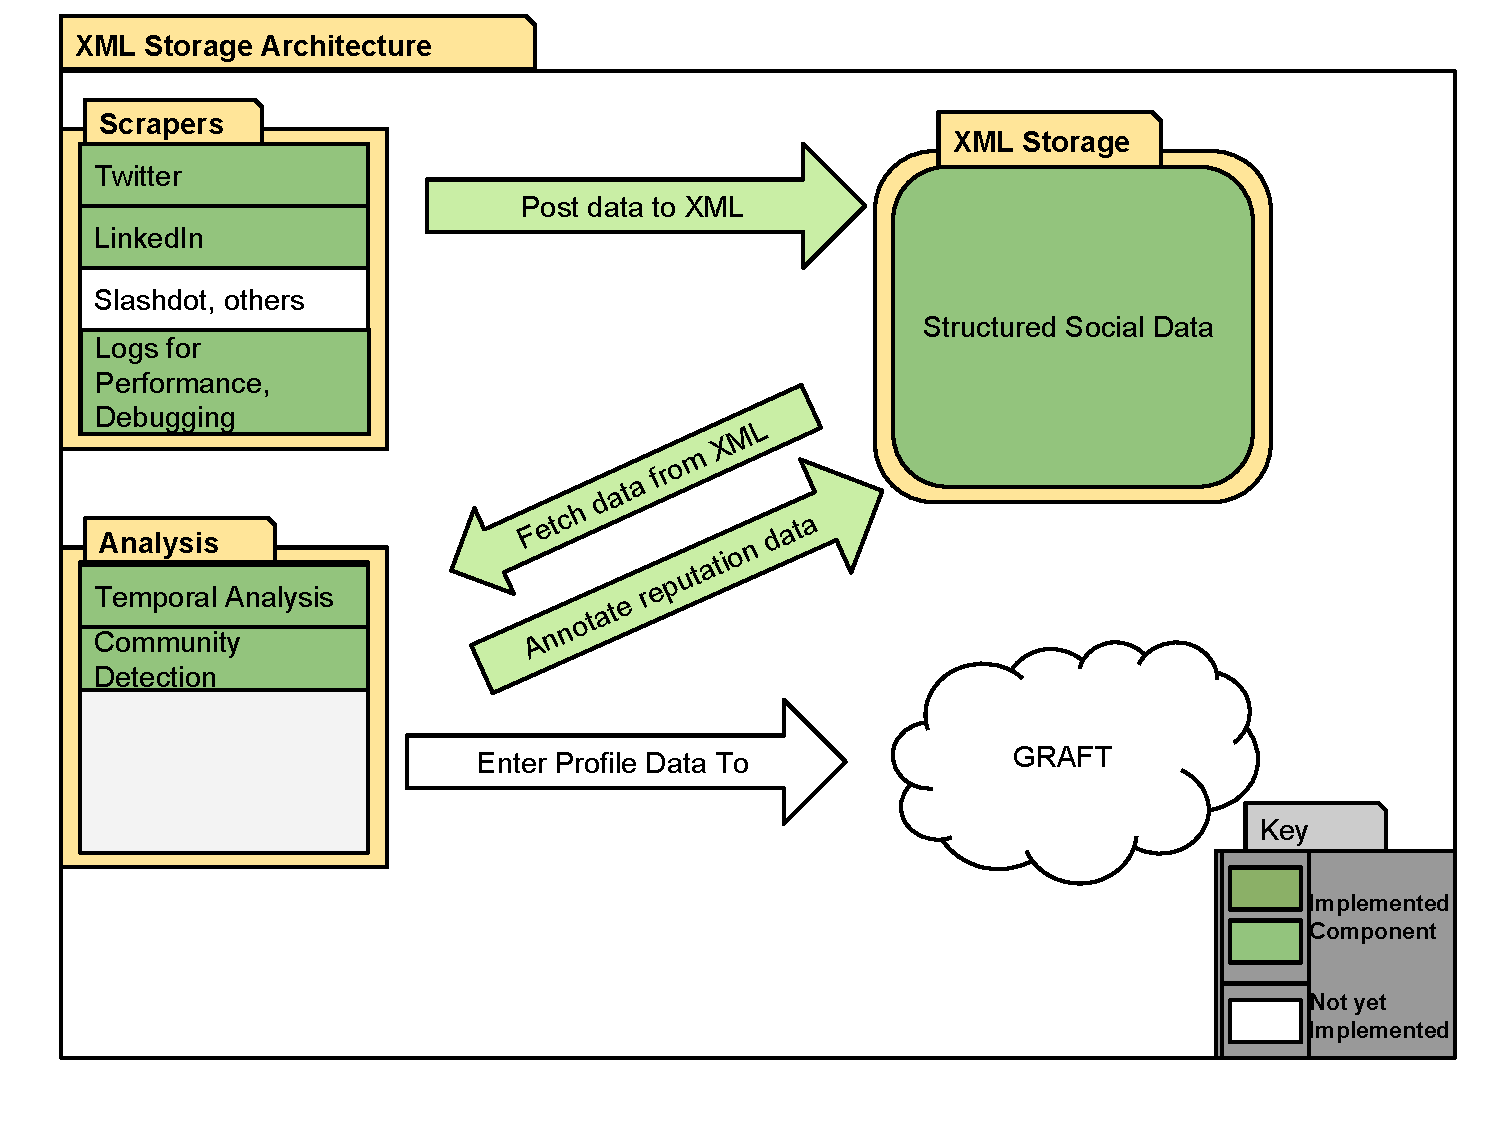
\includegraphics[width=0.9\textwidth]{Images/xml_storage_arch_v2.pdf}
\caption{Architecture for XML Storage Solution.}
\label{fig:xml_storage}
 \end{center}
\end{figure}
%File storage is also much faster and less server taxing than using a database
This design largely simplifies the scripting and scraper construction. Little setup was required during prototyping to construct schemas against which to save data. An informal XML approach also allowed for straightforward manipulation of data structures, and additions to what was being stored. Performance of storing to files is also known to be much faster and less server-taxing than the use of a database.

The primary disadvantage to the XML approach is difficulties associated with selecting individual slices of data in XML. Technologies such as xQuery exist for querying against XML, but were deemed unnecessary for the project. This is due to entire profiles being used for input into analysis components, rather than selected components only.

The text/XML design was used in the final solution. The time investment of setting up a database, as well as performance gains in using file storage over database storage were the primary contributors to this decision. The database approach was deemed to be over-engineered. 

\section{Framework Design}

Various framework design alternatives were considered when designing the IHPScrape framework. Four options were considered.

% I will discuss four options that were considered:
% 
% \begin{itemize}
%  \item Extend the scrAPI framework
%  \item Implement a browser-automation application
%  \item Use site APIs
%  \item Develop my own framework from scratch, using various Ruby Gems.
% \end{itemize}

\subsection{Extend scrAPI}
scrAPI is a Rubyforge project, allowing for fast implementation of web scrapers. The core benefit of scrAPI is allowing data to be fetched from HTML pages using CSS selectors. In addition it hides processes such as the actual fetching of pages. It is a much higher-level framework than what was eventually implemented.

Extending scrAPI was ultimately discarded, due to its heavy reliance on CSS files remaining constant. Any change to style sheet files would likely have broken the scrapers. Arguably these style sheets are less likely to change than layout manipulations (for example consider xpath on HTML as an alternative); however on sites such as Twitter and Facebook large design teams frequently make changes to these files. Given that requirement NF1 was to make scrapers resistant to user-interface change, this resulted in scrAPI being deemed unfit for purpose. 

\subsection{Extend A Browser-Automation Model}

Browser automation options were considered as an alternative architecture. Frameworks such as Watir \footnote{http://watir.com/} allow developers to simulate user interaction with web pages, by driving an actual browser instance.

A browser automated-scraper would likely have had little problem with site detection or blocking, due to the use of a real browser - providing genuine user agents, downloading CSS selectors and such. This would have been effective at fulfilling requirement F4. Despite this, performance would have been significantly poorer using this option, violating requirement NF2. As browser automation scripts are entirely dependant on site layout and interface naming conventions, this would have violated the requirement of resisting user interface change NF1. 

\subsection{Use the API}

A basic application interacting with the Twitter API was constructed early in the project. Twitter's API version 1.0 was actually highly suitable for the needs of the project. However the changes in REST API v 1.1 rendered this infeasible. The earlier API allowed fetching of up to 800 statuses from any public profile, along with more public data\footnote{https://dev.twitter.com/docs/api/1}. Version 1.1 however implemented more requirements for authentication, and limited functions such as downloading tweets to the individual's account only\footnote{https://dev.twitter.com/docs/api/1.1}. Facebook's developer API is even more restricted. On Facebook, permissions must be obtained from the appropriate users before fetching data from their profile. LinkedIn's policy is similar. %due to the changes!!!

\subsection{Implement a new Framework}

The fourth approach considered was to develop a new framework, built upon a number of Ruby libraries. This approach allowed for more flexibility when constructing scrapers, and consider new approaches to the user interface dependancies of web-scrapers. 

The primary disadvantage to this approach is the potential to re-implement work that has already been done previously. However by building the framework around existing libraries to perform the low-level networking technicalities of web-scraping, developer burden may be greatly lessened. This approach also allowed for development of a scraper framework tailored for social media, which was not present in frameworks researched.

% The most obvious disadvantage to this approach is the argument that by implementing my own scraping framework I was 'reinventing the wheel'. However by building the framework around existing libraries to perform the networking technicalities of web-scraping, I greatly lessen the developer burden. Also this approach allowed me to build a scraper framework tailored for social media, which was not present in frameworks I researched. 

%Advantages - flexibility, adapdability as I get to design and tune my own scraping framework. Can be built upon whatever libraries I choose. 

%Talk about why I chose to implement my scrapers using this method, and the advantages that this framework provides when considering the architecture.

The libraries upon which my scrapers were built included:

\begin{description}
 \item [Nokogiri]\footnote{http://nokogiri.org/}: a widely used HTML and XML parsing framework, allowing for straightforward interpretation of raw HTML documents. Nokogiri has many extensions, and can be effectively used to parse HTTP body responses into sensible HTML structure, which can then be parsed using xPath expressions to retrieve data of interest.
 \item [Mechanize]\footnote{http://rubygems.org/gems/mechanize}: an extension of the Nokogiri framework, that simulates browser actions on web-pages. 
 \item [Rest-Client]\footnote{https://github.com/rest-client/rest-client}: Ruby's most popular HTTP client. Rest-Client allows the use of all HTTP verbs, and can be adjusted for user-agent, proxy, and custom field input.
\end{description}

\begin{figure}[h!]
\centering
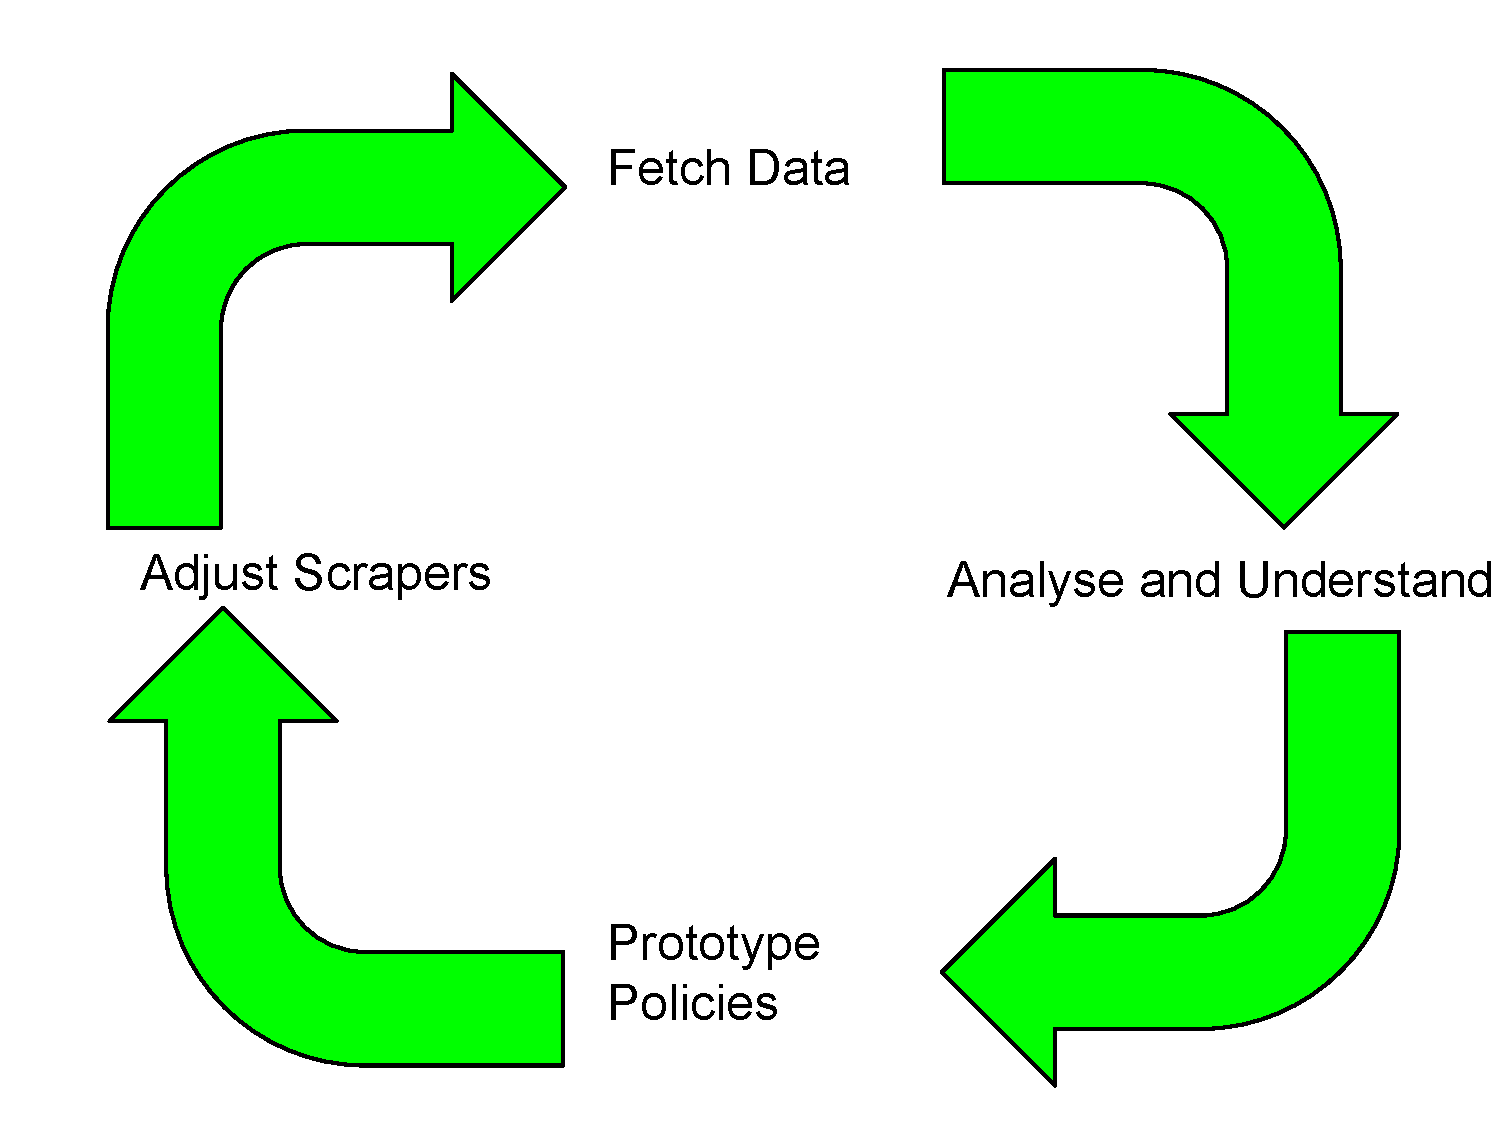
\includegraphics[width=0.4\textwidth]{Images/Implementation_Lifecycle.pdf}
\caption{Scraper Development Feedback Loop}
\label{fig:dev_cycle}
\end{figure}

\section{Framework Implementation}

Developing the project solution consisted generally of a cyclic, iterative prototyping approach as detailed in Figure \ref{fig:dev_cycle}. This generally consisted of four phases; implementing and adjusting scrapers, fetching data, analysing the data, and prototyping policy concepts as a result of this analysis. 

\section{Technology}

The web-scraper components were written entirely in Ruby. The development of screen scrapers is largely independent upon language choice; however Ruby was selected due to its large number of libraries suitable for scraping, and straightforward scripting nature. Ruby also has a significant Open Source following in comparison to many more conventional languages like Java. This was considered necessary early in the project, when looking at a model for future maintenance of the scrapers, especially for the discarded requirement of aggregating data for GRAft. 

Alternatives to Ruby were considered; Java, which does not have the same open source following as Ruby, as well as a larger degree of lower-level network coding for web-scraping software; and PHP, which was rejected due to time constraints limiting personal capabilities to learn the language to a competent level during the project. PHP would have given the advantage of being more consistent with past works, however \cite{GRAft}, as well as being the same language as my policies are described in. This is just a 'nice-to-have' feature however, and would not have added any real value to the project design.

\section{IHPScrape Framework}

The IHPScrape framework was implemented as per the architecture in Figure \ref{fig:xml_storage}. The purpose of the framework was to outline a class structure for following scrapers, as well as abstract the low level networking request details which all scrapers had to implement. 

%

Talk about the development of a generic scraping framework, and the considerations put in place during the this development.

Request Handler generic request writer which is able to handle errors, etc. General layout for scrapers which scrapers implement.

Talk about xPath somewhat, as a language to select items from page from.


%\begin{figure}[h!]
%\centering
%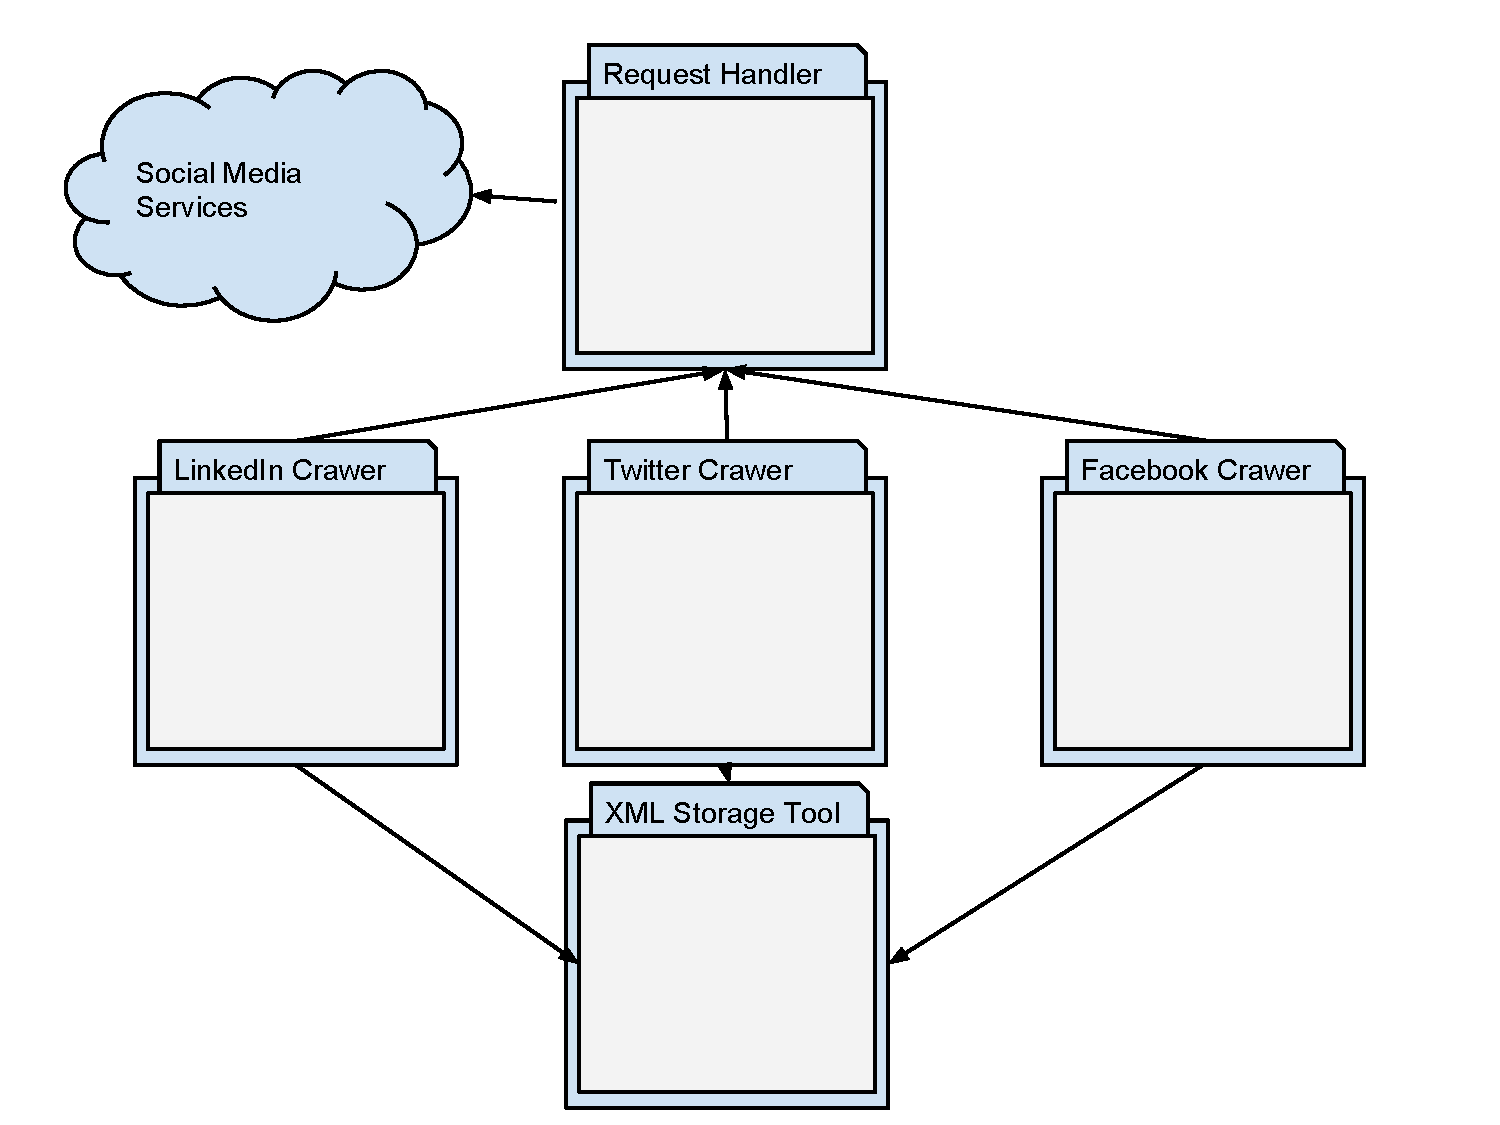
\includegraphics[width=0.6\textwidth]{Images/Code_Reuse.pdf}
%\caption{Pipes-and-Filters Class Structure}
%\end{figure}

\section{Facebook Crawler}

A Facebook scraper was prototyped early in the project, and allowed for experimentation with many of the technologies that were used later. Firstly, strategies for authenticating against Facebook had to be developed. While public profiles do exist, these are primarily for company pages or politicians, which is not what the project aimed to solely investigate. Authentication was implemented using a dummy Facebook account, through the Mechanize Ruby framework. Mechanize allows for form data on pages to be populated and submitted through either HTTP or HTTPS. Once authentication was achieved, an authentication token was passed as an attribute of further requests. New authentication tokens are obtained after an adjustable time period, or on a new scraper run. 

Having obtained the necessary authentication tokens, profile pages could be fetched. The planned approach was to crawl through friend networks via friend lists, and scrape profiles in this manner. Downloaded profiles would then be parsed using Nokogiri, and relevant data extracted via xpath expressions. Posts, likes and friend lists are examples of information identified as useful to collect. However as mentioned in Chapter 3, this scraper was eventually discarded as infeasible. Scraping large amounts of content reliably through Facebook was infeasible within the project's scope due to its highly dynamic content, and frequently changing interface. Maintaining and updating a scraper to fetch accurate data from Facebook during the project would have been too time-consuming and as a result was removed from the project scope. However the technologies experimented with whilst developing this prototype were useful later when developing the more robust Twitter scraper.

%Discuss what I built the Facebook prototype with. Then mention that the technologies used here were added to in order to make the Twitter Crawler. Discussion as to why this was discarded as a requirement.

\section{Twitter Crawler}

The Twitter Crawler users a Google Twitter search function to search for profiles to fetch at the top level. An input text file of random names delimited by lines is accepted by the scraper. These names are looped through in order, with the scraper fetching the profiles of these top ten results returned through Google. Bias is introduced through this approach, since only the top ten search results are analysed. 

%The Twitter Crawler uses a Google Twitter search function, to loop through profiles at the top level. An input text file of random names delimited by lines is accepted by the scraper. These names are looped through in order, with the scraper fetching the profiles of the top 10 results returned through Google. Bias is introduced through this approach, as results appearing in Google are naturally more popular than users who would not. However as the top ten results are fetched and prepared for scraping, in general the lower ranking users here are more 'standard'. 

Due to this bias, alternative approaches were considered. A potentially better scientific approach to randomising the selection of profiles to scrape would have been to crawl through an already-generated set of random profile names. However searches did not reveal any such databases to exist, excluding celebrity-exclusive ones which would have been significantly worse than my current approach. Crawling via embedded links on Twitter was also considered, starting from any profile and following re-tweet links through to new profiles. However this introduces new complexities such as detecting infinite loops (potentially very large), or detecting repeated profiles. As the project was ultimately about reputation and not scraping algorithms, the simple name-searching approach was selected. 

Once the ten profile names are selected (for the current input name in the text file), the application will perform the scraping of each of these profiles in order.  The definition of a Twitter profile changed throughout the project, as more information was chosen to be analysed. The final schema of stored data for the standard Twitter scraper is contained in appendix 1.1. Essentially all tweets are captured where possible, along with associated re-tweets, favourites, and the profile names of users who re-tweeted this item. Profile meta data is also stored, such as number of followers, number following, and total number of tweets. 
%CHANGE THIS AS APPROPRIATE. 

A number of technical difficulties exist with fetching such profiles and meta data. Firstly, a Twitter page does not immediately display all tweets for a user for obvious loading reasons. To view more than the initial tweets, users must scroll through an \textit{infinite scrolling} window which requests more data through AJAX calls. To simulate this interaction, I used Google Chrome's \textit{network capture} feature to inspect requests to the page during the scrolling function. A max\_id parameter in the URL is adjusted to modify the tweet window fetched.

% The URL is of the following form:
% 
% \begin{verbatim}
%  /timeline/with_replies?include_available_features=1&include_entities=1&max_id=12345
% \end{verbatim}

The JSON returned is then parsed to retrieve relevant information. As a Twitter profile may contain re-tweets from other profiles, checks have to also be taken at this stage to ensure the content is originally generated by the user of interest. This is as simple as checking the user name who posted the content originally. In order to increase the performance of extra tweet fetching, various tweet window sizes were experimented with. This was ultimately ineffective at maximising speeds.

\subsection{Parallel Tweet Fetching}

Although tweet content can be fetched from the base profile page, useful data such as re-tweet and favourite count is initially hidden. To view tweet detail, a further request must be sent, to mimic the user interaction of clicking on the tweet. Fortunately this process can be parallelized for each tweet within a tweet window. In the final twitter scraper a thread pool of 15 threads is created, one for each potential tweet in the window. Each thread then fetches and parses each tweet individually. To ensure parallel performance is not lost, any tweet-fetching process that fails here will simply be thrown away. Parallelization of tweet fetching resulted in huge performance gains. Parallel fetching was not considered earlier in the project as I expected the resulting simultaneous requests to end in more frequent detection by sites. 

\subsection{Detection Avoidance and Recovery}

Operating on the University network likely resulted in less chance for blocking detection by Twitter, due to the large IP range allocated to Victoria University. Regardless, steps were taken to limit detection rates. Multiple strategies for avoiding detection were considered, and several employed simultaneously. The Request-Handler package handles the implementation of these strategies.

The first and most straightforward strategy is to include random pause times between requests. The goal of this approach is to reduce potential server burden, and lessen the possibility of an aggressive scraper being permanently blocked due to its flooding the site. However this approach imposes a very low ceiling for performance and tweet fetch rates. It is recommended to leave a ten to fifteen second delay between requests, but such a pause was infeasible for the needs of the project \cite{howto_scrape}.As such, pauses between requests were only implemented in certain special cases; failed requests and at the end of a profile. 

The second strategy employed is to send requests that spoof a browser user-agent, in order to appear as a legitimate browser instance at the server end. Before scraping a new tweet window, a new user-agent string is randomly selected from a list. 

A third strategy that was considered but not implemented was the downloading of CSS and other markup, in order to behave as browser-like as possible. This was discarded because of questions of its feasibility, as well as uncertainty as to the level of potential benefits from constructing such a solution. 

%Rate limiting detection
I rarely encountered rate limiting at University, and was never blocked outright on the University machines. Early in the project, when prototyping a Facebook scraper I was briefly banned from Facebook at home. 503 errors (indicating resource unavailability) reveal detection on Twitter. 500 errors (indicating server error)  were encountered throughout the project also, but these were due to coding errors. 

\subsection{Authentication}

The original scraper did not require authentication, since the majority of Twitter profiles are viewable to individuals who do not have a Twitter account, or are not signed in. However to fetch the names and profiles of users re-tweeting posted content, an authentication feature had to be added. Fortunately the authentication strategy employed by the Facebook prototype was able to be re-used for this component. The same strategy as constructed for Facebook of logging into a dummy account at the beginning of a scraping run was used.  

\subsection{Parsing Poorly Formed Markup}

An initial concern was the scraping of content containing poorly formed HTML or JSON markup. Thankfully the sensitivity of HTML parsers to poor markup is largely library-dependant. This was not well-documented in the gems found, so experimentation with various options had to suffice. Nokogiri was sufficient for HTML parsing, and the default ruby JSON parsing library was most effective at parsing incomplete JSON data.

%Mention that the code is available from github. http://www.github.com/irwalker/dat-roll

%Content behind login

%Infinite scrolling

%Rate limiting -> encountered sometimes? 503 errors primarily

%'Scraper window', not actually very effective, due to the primary networking burden being on sending a separate HTTP request to download every tweet.

%Spoofing headers -> using fake user-agents, and rotating between user agents in between overall requests.

%Poorly formed markup -> was an occasional issue. Found that some libraries were more strict on this than others, and adjusted accordingly.

%Authentication

%Pattern scraper employed to fetch data. 

\section{LinkedIn Scraper}

The LinkedIn Scraper was developed towards the close of the project, and as a result data analysis of what was collected using this tool was not carried out. However developing this tool, which is able to scrape multiple LinkedIn profiles in parallel, was able to prove the extensibility of the IHPScrape framework in the context of a new social media site. The LinkedIn scraper was developed in one week's construction time. This was much less time than was spent developing and debgguing the original Twitter scraper and framework, and is evidence of the portability of the framework. However consideration must be given to the simplicity of the LinkedIn website as compared to Twitter. Also, the first iteration of my Twitter scraper only took approximately two and a half weeks (this build did not include the infinite scroll scraping feature). 

%The time to develop the LinkedIn scraper, including implementing parallel profile fetching totalled 3 days work. This was weeks less time spent

%Discuss how the implementation of this component was a success in that it proved the extensibility of the framework developed. 

%brief description of the work done developing the LinkedIn scraper. What was fetched, etc etc.

\section{Code instrumentation}

The code was instrumented using a Ruby logger system written for the application. Given complexities and difficulties debugging errors on web-scraping applications, logging had to be performed to a very fine level of granularity. Any action changing system state such as fetching a page triggers the logging mechanism. The logger would then take note of the timestamp and write to the appropriate file the nature of the action. For example, if the scraper sent an HTTP request to retrieve a given URL, it would record the timestamp and URL requested. 

The logger would write to the appropriate log file based on the nature of the supplied action. Because these scrapers were running over long periods of time, using traditional IDE debugging tools was not effective at detecting errors. As a result, multiple debugging files with different purposes were used in an attempt to catch these errors. The debug log captured all interaction information at a basic level. The error log captures error information that is non-fatal to scraping an individual's profile, e.g. on Twitter. Commonly these errors were due to application logic flaws, such as performing operations on null entities. As a result the error log assisted greatly in identifying these edge cases. Finally the failure log was used to record fatal exceptions that would prevent me from scraping a profile. Occurrences such as 404, 500 or 503 responses from servers are examples that would result in a record being written to the failure log. The failure log would write system state at the time of failure to a high level of detail, sometimes even writing the entire HTML document before the failure to disk. This again assisted with debugging, when reviewing how a particular run had gone. 

To limit the performance overhead of writing to these logging files, a buffered approach was taken in order to achieve the least impact. 

\section{IHPScrape Summary}

Write a summary of the scrapers here yo. Made a Framework which can be applied to multiple social media sites. Implemented for Facebook Twitter and LinkedIn, but Facebook was discarded due to its too often changed user interface. 

%lol
